\documentclass[journal]{IEEEtran}

% *** CITATION PACKAGES ***
%
%\usepackage{cite}
\usepackage{capt-of}%%To get the caption
\usepackage{gensymb}
\usepackage{graphicx} %package to manage images
\graphicspath{ {./images/} }
\usepackage{wrapfig}

\usepackage[style=ieee]{biblatex}
\DeclareLanguageMapping{english}{english-apa}
\addbibresource{references.bib}
\usepackage[justification=centering]{caption}

\usepackage{setspace}

\usepackage{hhline}

\usepackage{booktabs}

% *** GRAPHICS RELATED PACKAGES ***
%
\ifCLASSINFOpdf
  % \usepackage[pdftex]{graphicx}
  % declare the path(s) where your graphic files are
  % \graphicspath{{../pdf/}{../jpeg/}}
  % and their extensions so you won't have to specify these with
  % every instance of \includegraphics
  % \DeclareGraphicsExtensions{.pdf,.jpeg,.png}
\else
  % or other class option (dvipsone, dvipdf, if not using dvips). graphicx
  % will default to the driver specified in the system graphics.cfg if no
  % driver is specified.
  % \usepackage[dvips]{graphicx}
  % declare the path(s) where your graphic files are
  % \graphicspath{{../eps/}}
  % and their extensions so you won't have to specify these with
  % every instance of \includegraphics
  % \DeclareGraphicsExtensions{.eps}
\fi
% graphicx was written by David Carlisle and Sebastian Rahtz. It is
% required if you want graphics, photos, etc. graphicx.sty is already
% installed on most LaTeX systems. The latest version and documentation
% can be obtained at: 
% http://www.ctan.org/pkg/graphicx
% Another good source of documentation is "Using Imported Graphics in
% LaTeX2e" by Keith Reckdahl which can be found at:
% http://www.ctan.org/pkg/epslatex
%
% latex, and pdflatex in dvi mode, support graphics in encapsulated
% postscript (.eps) format. pdflatex in pdf mode supports graphics
% in .pdf, .jpeg, .png and .mps (metapost) formats. Users should ensure
% that all non-photo figures use a vector format (.eps, .pdf, .mps) and
% not a bitmapped formats (.jpeg, .png). The IEEE frowns on bitmapped formats
% which can result in "jaggedy"/blurry rendering of lines and letters as
% well as large increases in file sizes.
%
% You can find documentation about the pdfTeX application at:
% http://www.tug.org/applications/pdftex

\begin{document}

\begin{titlepage}
    {\centering
        \vspace*{20em}
        {
        \huge 
        \begin{spacing}{1.5}
            Lab Report \#6: Operational Amplifier (Opamp) Circuit
            \\
            Circuits Fundamentals Lab, Spring 2019
            \bigskip
            \Large
            \\
            Determining the Characteristics of an\\
             Operational Amplifier (Opamp)
  
            \\
            \bigskip
            Deadline: March 13, 2019 
        \end{spacing}

        }
        
    }
    \vfill
    
    {
    \large
    
    \begin{spacing}{1.5}
    \noindent Barkin Simsek, {\it {bs3528@nyu.edu}} 
    \\
    Nishant Aswani, {\it {nsa325@nyu.edu}}
    \\
    Section \#1% <-this % stops a space
    \\
    Workstation \#8% <-this % stops a space
    \end{spacing}
    }


\end{titlepage}
\pagenumbering{gobble}
%\clearpage\mbox{} % adds and empty page
%\clearpage
\pagenumbering{arabic}
\setcounter{page}{1}

%\title{Demonstration of a Voltage Divider With A Variable Resistor}

%\author{Barkin Simsek,~\IEEEmembership{bs3528@nyu.edu};
%Nishant Aswani,~\IEEEmembership{nsa325@nyu.edu}
%\\ Table Number: \#}% <-this % stops a space


% The paper headers
\markboth{Simsek, Aswani, Circuits Fundamentals Lab 2019}%
{}

% make the title area
%\maketitle

% As a general rule, do not put math, special symbols or citations
% in the abstract or keywords.
\begin{abstract}
In this experiment, an opamp amplifier circuit was built by using a Texas Instruments LM386 opamp. The built circuit is capable of providing a voltage gain of 200. The circuit was initially built onto a breadboard and later the circuit was soldered on to a prototyping board. Providing an extreme input voltage, providing an extreme frequency, and providing a low supply voltage each had determinetal effects on voltage output, and thus gain. It was determined that the produced circuit can be used to increase the signals in a radio receiver and is ideal for audio applications.
\end{abstract}

%Percenta of power being consumed at the internal resistence

%What happens to voltage when external load is connected and current %consumption increaased

%Formula derivation
%Application 


\section{Introduction}

\IEEEPARstart{T}\lowercase{he} goal of this lab was to prototype and build a circuit using an operatonal amplifier, in order to attain a gain of 200.\\ 

% \noindent As current passes through the coil in the inductor, a magnetic field, and thus a magnetic flux, is generated through the core. Increasing or decreasing the current, produces a change in the magnetic field, which is followed by the generation of an electric field \cite{inductors}. Thus, while an inductor acts as a short-circuited wire to direct current (DC), the main quality of the passive component is that it opposes the changing of current direction through it \cite{hayt1986engineering}, which is what alternating current (AC) provides. Following this, an inductor is incapable of having an abrupt or non-continuous change in current passing through it. Moreover, looking at equation \ref{eq:inductorTheory}, an infinite change in current would require an infinite voltage, which is physically impossible.

\noindent An operational amplifier (opamp) is a circuit component often used for signal conditioning, part of which involves signal amplification. Thus, opamps are often used to produce a greater output voltage compared to the input voltage. The external components and connections can also be manipulated to increase voltage and current given either current or voltage \cite{basicOpAmp}, making opamps one of the most versatile circuit components.\\

\noindent This lab focused on the LM386 opamp designed by Texas Instruments (TI). TI describes the component as a "power amplifier designed for use in low voltage consumer applications" \cite{tidata}. While the internal gain is set to 20, the company claims that "the addition of an external resistor and capacitor between pins 1 and 8 will increase the gain to any value from 20 to 200" \cite{tidata}. The LM386 opamp is most commonly used for amplifying sound by increasing the gain, which defined as the ratio between voltage output and voltage input.


\begingroup
    \centering
    \medskip
    %width=\columnwidth
    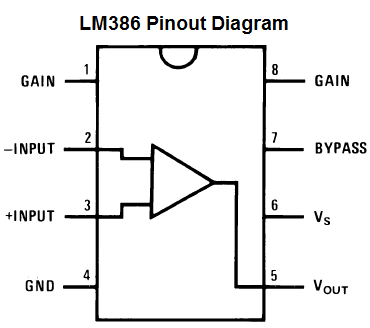
\includegraphics[scale=0.6]{images/lab6_1.png}
    \captionof{figure}{Pinout diagram of the LM386 opamp}
    \label{fig:pin}
    \medskip
\endgroup

\noindent As shown by Figure \ref{fig:pin}, the opamp has 8 pins. Pins 2 and 3 are used for input voltage, usually a low signal to be amplified, while Pin 6 is for supplying the opamp and its components with power, in this case 9V. Pin 5 is used to obtain the output conditioned by the opamp. In this application, where the goal was to achieve a gain of 200, the circuit schematic shown in Figure \ref{fig:circuit} was used. 

\section{Prototyping and Building the Circuit}

\noindent Following the schematic above (Figure \ref{fig:circuit}), the circuit was initially recreated on a breadboard. The positive (VCC) and

\begingroup
    \medskip
    \centering
    %width=\columnwidth
    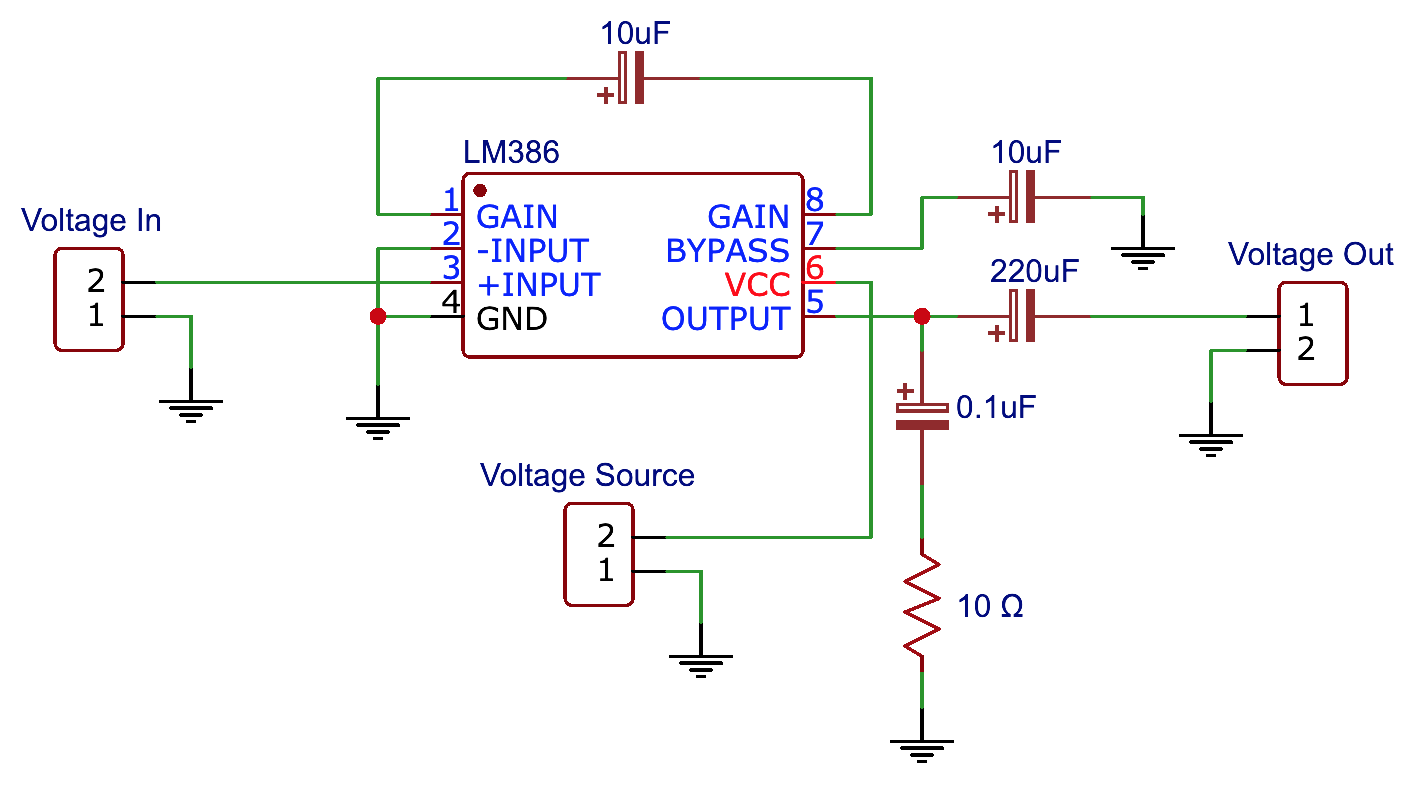
\includegraphics[width=\columnwidth]{images/lab6_2.png}
    \captionof{figure}{Circuit schematic for the LM386 to obtain a gain of 200}
    \label{fig:circuit}
        \medskip
\endgroup

 \noindent negative (GND) terminals were attached to the appropriate power rails on the breadboard, which were then wired to Pins 3 and 2, respectively. The power supply, set to 9V, was connected to pin 6. The two legs of 10 $\mu$F capacitor were connected to pins 1 and 8. Leg one of another 10 $\mu$F capacitor was attached to pin 7 and the other leg was grounded. Finally, a 220 $\mu$F capacitor was connected to pin 5 and a $V_{out}$ with a 0.1 $\mu$F with and 10\ohm resistor connected in parallel. \\

\noindent Once the circuit connection and operation was confirmed on the breadboard, the components were soldered onto a prototyping board. As a replacement to the power rails, through which voltage was inputted and outputted, the soldered board made use of screw terminals. Figure \ref{fig:board1} and \ref{fig:board2} depict the final result after soldering all required components.\\

\section{Results}

\noindent After building the circuit, several conditions were tested, all of which are outlined in Figure \ref{fig:table} below. The first check was to confirm whether the soldered circuit was operational and whether it provided the expected results.\\

\noindent To calculate the gain, $ V_{out}$ was simply divided by $V_{in}$. $V_{in}$ was varied by varying the input voltage  in pin 2, while frequency was varied by varying the input frequency in pin 2. The $V_{s}$ was varied by varying the input voltage into pin 6.\\


\begingroup
    \medskip
\centering
\def\arraystretch{1.5}
\begin{tabular}{cccccc}
\toprule
& T1 & T2 & T3 & T4 & T5 \\
\midrule
$V_{in}$ (V) & 0.02 & 1 & 0.02 & 0.02 & 0.02 \\
$V_{out}$ (V) & 4.08 & 8.6 & 4.4 & 3.4 & 0.03 \\
Gain & 204 & 8.6 & 220 & 170 & 1.5 \\
Frequency (Hz) & 10k & 10k & 1k & 200k & 10k \\
$V_{s}$ (V) & 9 & 9 & 9 & 9 & 1 \\
\bottomrule
\end{tabular}
\captionof{figure}{Tabulation of the collected data given the various settings per trial}
\label{fig:table}
    \medskip
\endgroup


\begingroup
    \centering
    \medskip
    %width=\columnwidth
    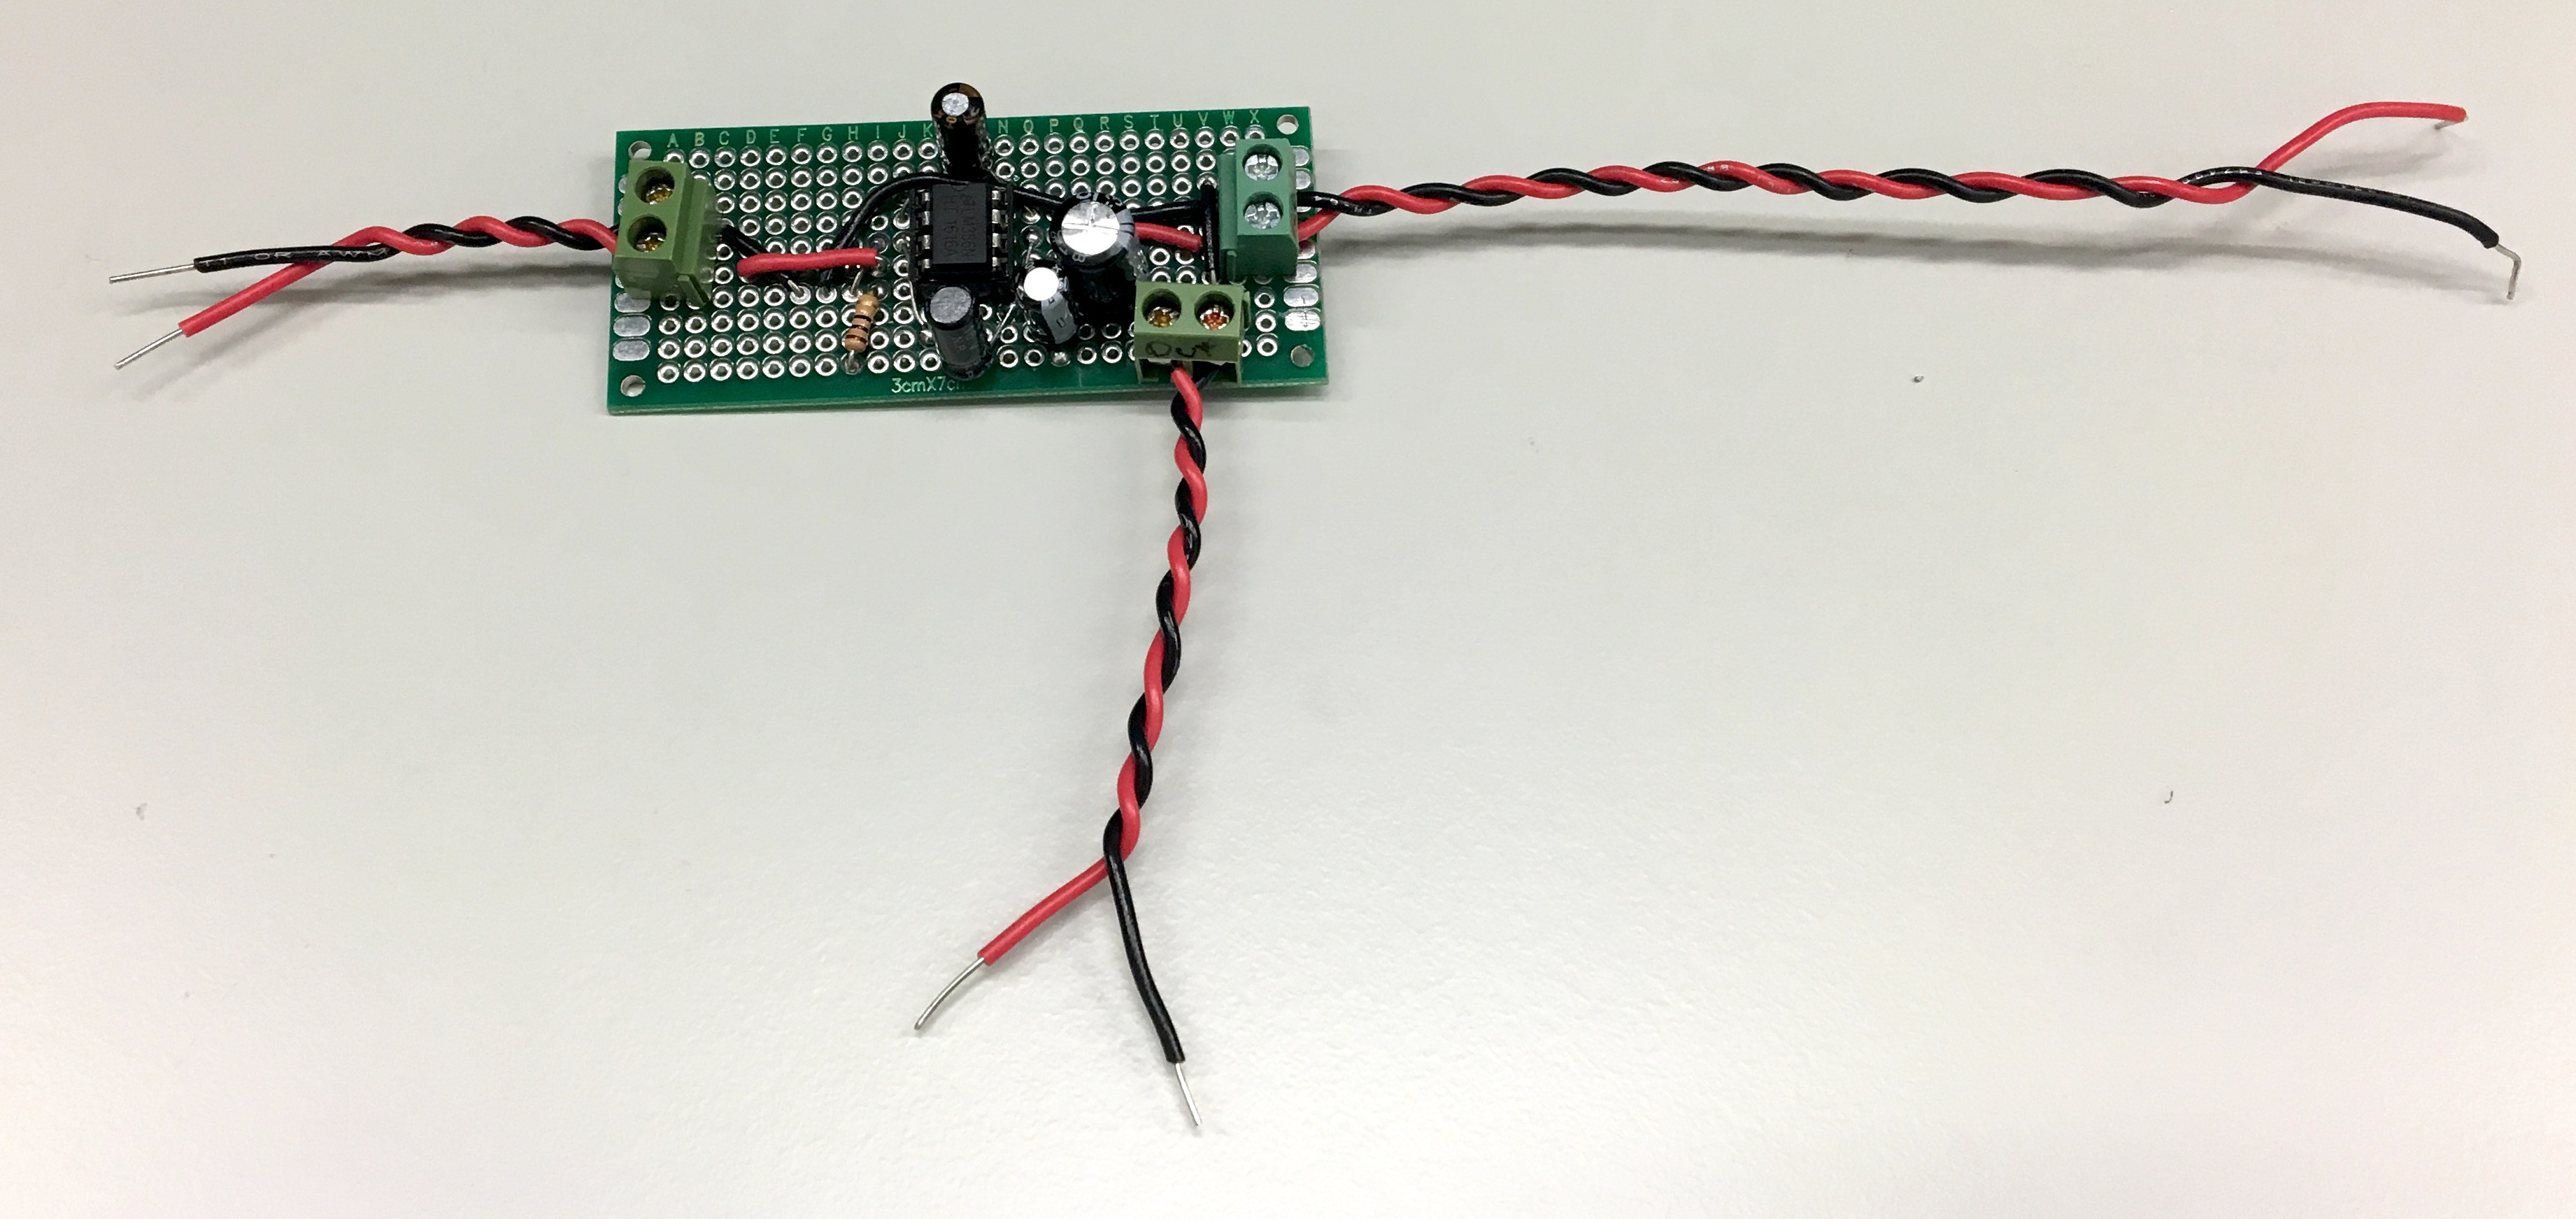
\includegraphics[width=245]{images/lab6_4.JPG}
    \captionof{figure}{Soldered board consisting of capacitors, resistors, the opamp chip, and screw terminals}
    \label{fig:board1}
    \medskip
\endgroup

\begingroup
\medskip
    \centering
    %width=\columnwidth
    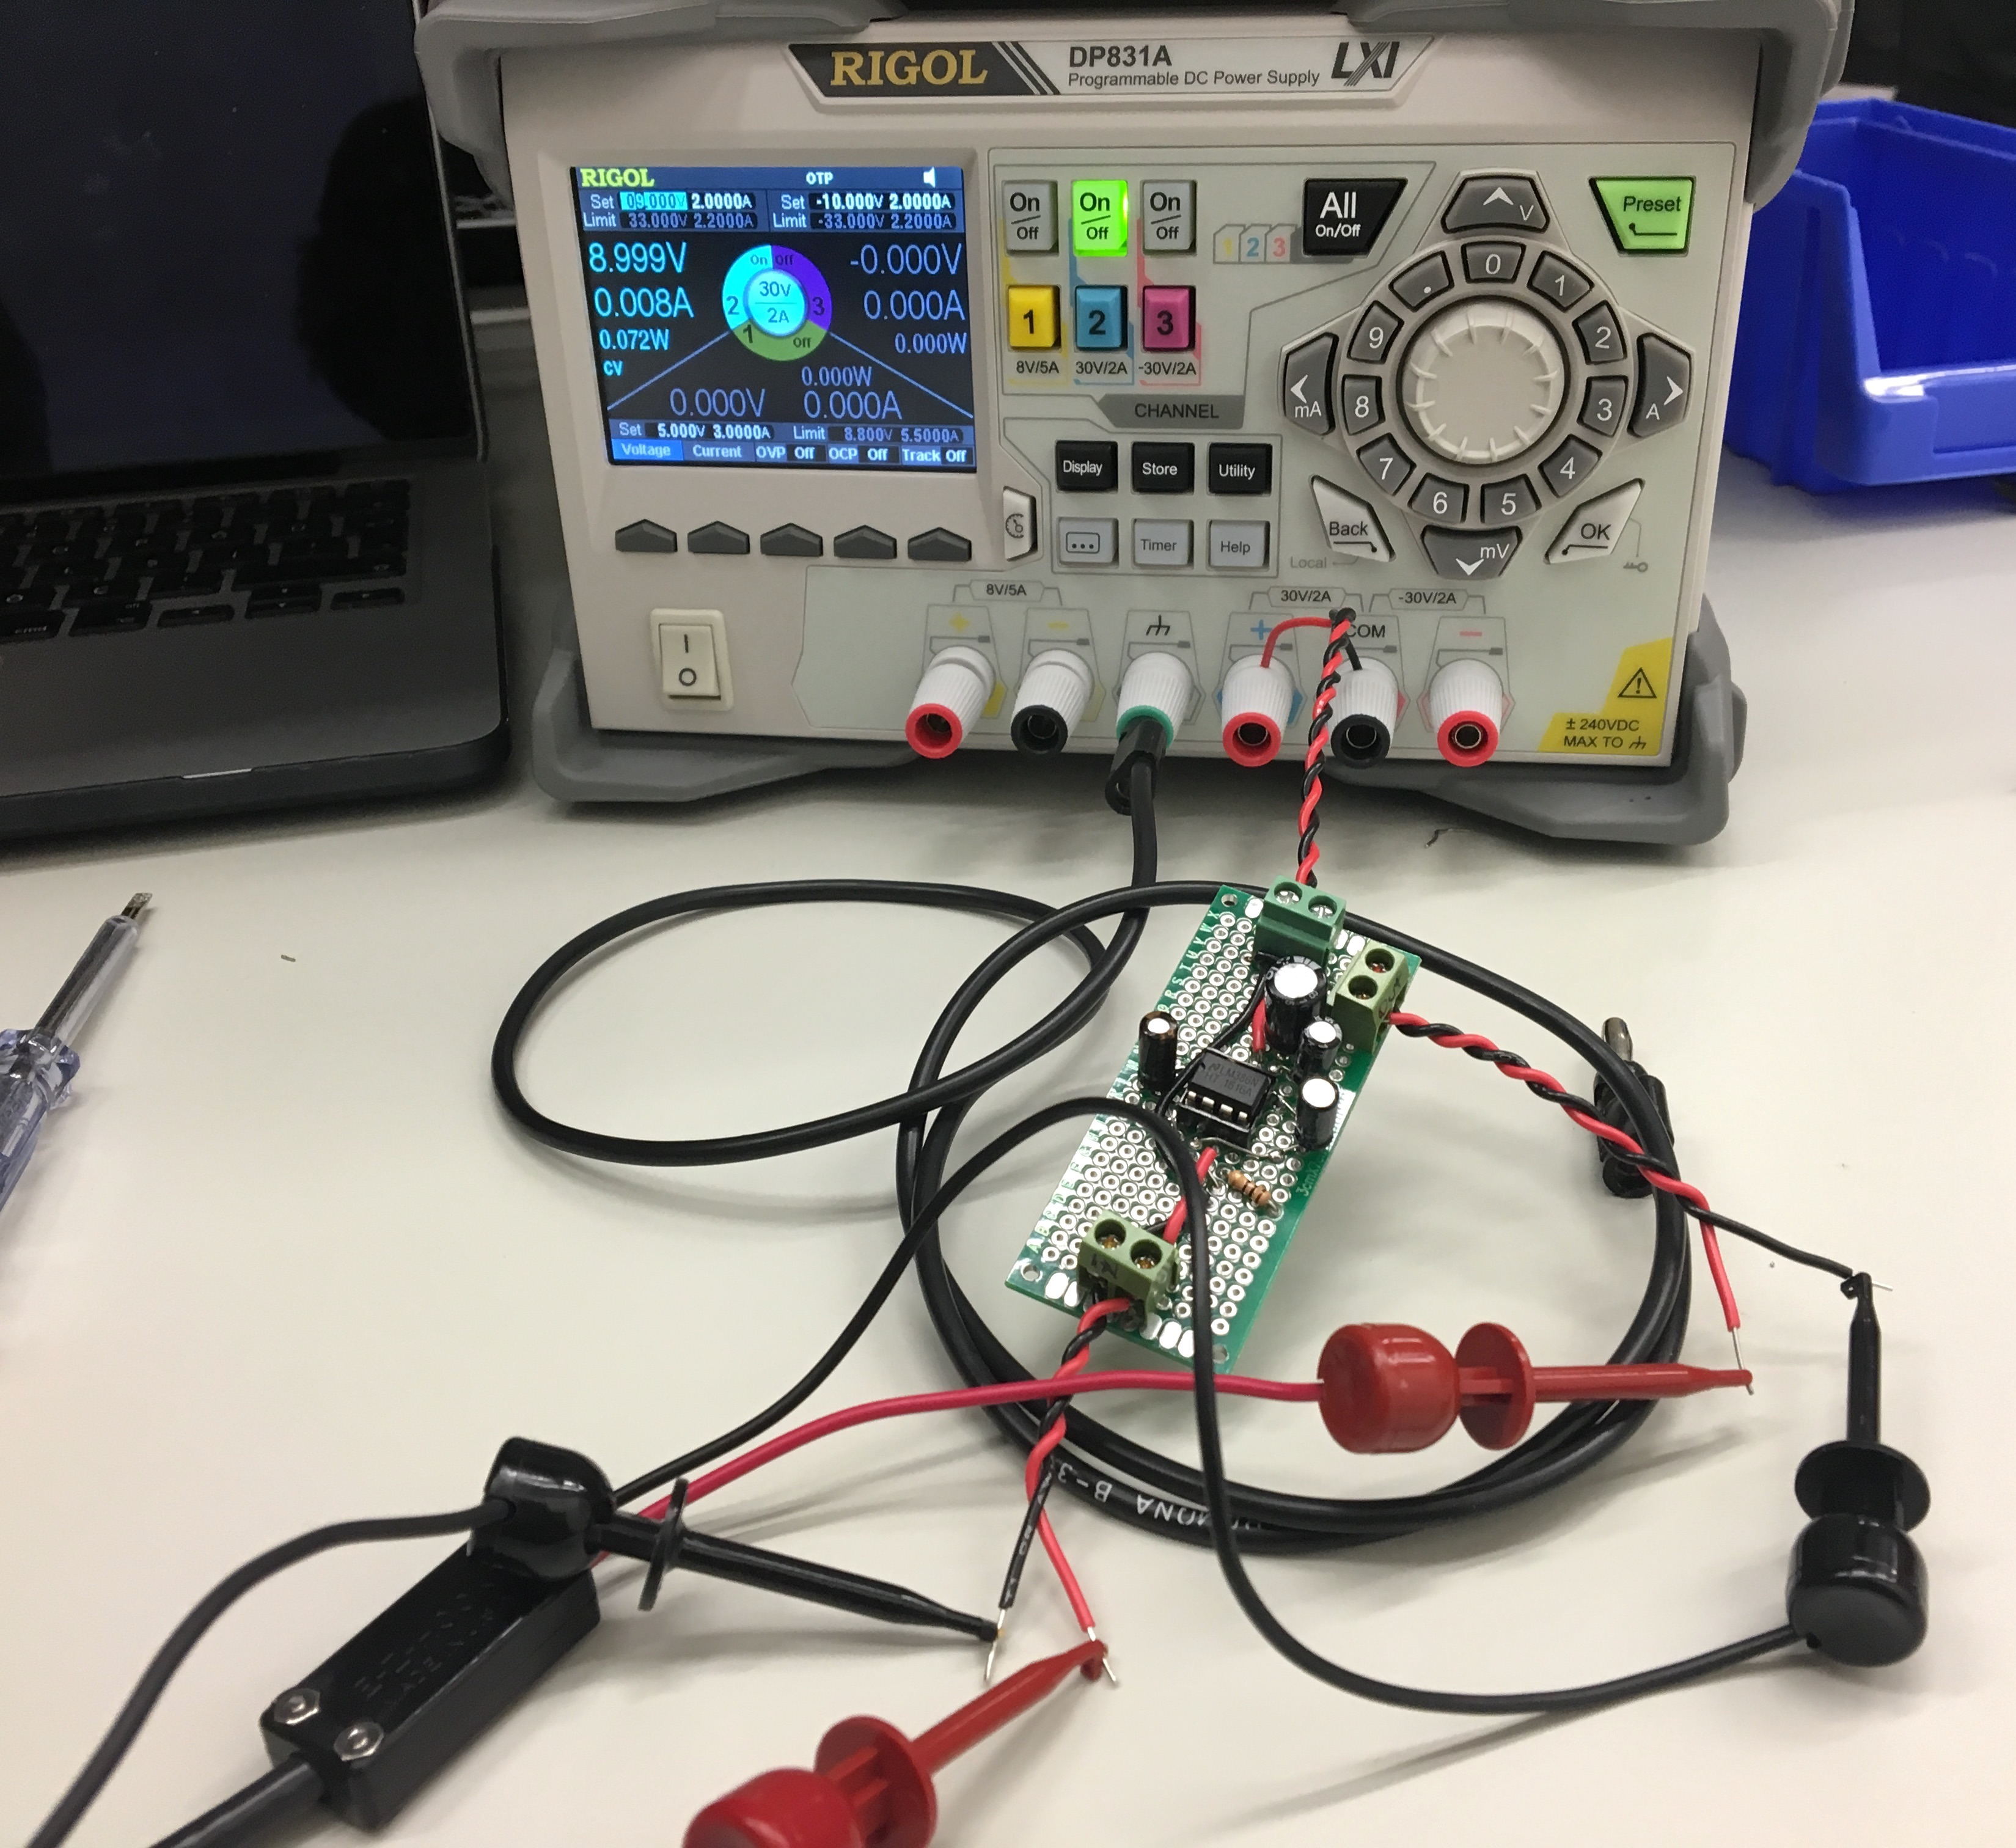
\includegraphics[width=245]{images/lab6_3.JPG}
    \captionof{figure}{Connecting the voltage amplifying board with a power supply of 9V}
    \label{fig:board2}
    \medskip
\endgroup

\section{Discussion}

\noindent Comparing T1 and T2, the only difference in the input is the increase in input voltage from 20 mV to 1V; as a result, the gain is far lower in the second scenario. Although the opamp circuit is designed to provide a gain of 200, the opamp is only able to provide a maximum output of approximately 10 V \cite{tidata}. Therefore, limited by the opamp, the circuit is incapable of providing the theoretical 200V in output. Continuously providing the chip with 1V input would have most likely damaged the opamp, as its maximum rating is for 0.4V.\\ 

\noindent In scenario T3, the frequency is changed from 10kHz to 1kHz, resulting in a slight increase in output voltage and thus gain; however, this change in gain is not appreciable. On the other hand, changing the frequency from 10kHz to 200kHz, as in T4, results in a much more significant change in gain. The result for this change in gain is due to the opamp's frequency bandwidth. The frequency bandwidth of an opamp refers to the frequency range in which gain remains stable; if the frequency is extremely high or extremely low, then the gain begins to gradually drop (see Figure \ref{fig:curve}). However, in the case of a 200kHz frequency, the drop in gain does not matter because it is outside the human audible range of 20Hz to 20kHz, especially since the opamp is used for audio purposes. In fact, the opamp is designed to have a frequency bandwidth lay within this range because the LM386 is primarily used for audio purposes. Manufacturers also tend to decrease the cut off range to improve stability; this can often be done by adding capacitors networks within the opamp itself.

\noindent In the final T5 scenario, bringing the frequency back into the opamp's range and ensuring that input voltage is reasonable, but decreasing the supply voltage from 9V to 1V, leads to a severe drop in gain. As is shown in Figure \ref{fig:supply}, it is clear that decreasing the power supply to the opamp reduces the performance of the component, thus preventing it from providing its maximum possible gain. 

\begingroup
\medskip
    \centering
    %width=\columnwidth
    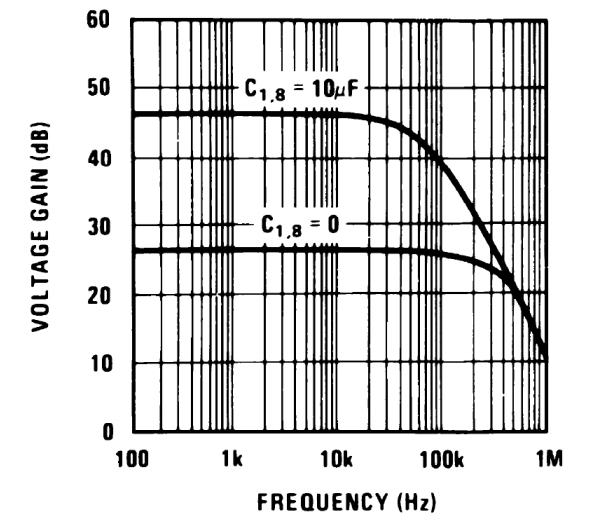
\includegraphics[width=245]{images/lab6_5.png}
    \captionof{figure}{Frequency response curve of the LM386 \cite{tidata}}
    \label{fig:curve}
    \medskip
\endgroup

\begingroup
\medskip
    \centering
    %width=\columnwidth
    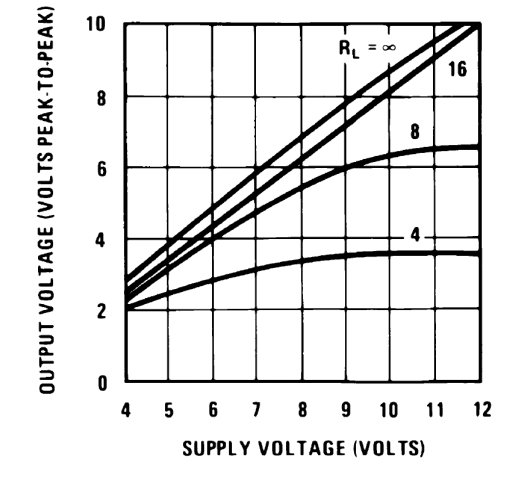
\includegraphics[width=245]{images/lab6_6.png}
    \captionof{figure}{Output voltage compared to the supply voltage \cite{tidata}}
    \label{fig:supply}
    \medskip
\endgroup

\section{Conclusion}

\noindent Opamps are circuit components most commonly used for signal conditioning, which can refer to increasing the output voltage or current of an input signal. In this exercise, an opamp circuit, capable of providing a voltage gain of 200, was built using the recommended components from TI's data sheet. The components were first tested on a breadboard and then soldered onto a prototyping board. Various scenarios were tested with the soldered board (varying input voltage, frequency, and supply voltage). It was determined that providing an input voltage too great would damage the opamp according to the data sheet but would also not lead to maximum gain the circuit can produce, because there is a limit to the output voltage on the opamp. Secondly, it was discovered that the opamp provided the desired gain within a certain frequency, known as a frequency bandwidth, beyond which the gain drops. However, the LM386 being an opamp with audio applications, is designed to provide maximum gain in the human audible range. Finally, it was determined that decreasing the supply voltage would prevent the opamp from operating at its full, thus compromising the voltage gain.\\ 

\noindent The LM386 opamp can be used as an audio amplifier in guitar amps or speakers. The fact that the LM386 requires only a 9V power supply, and is thus a low power consuming device, makes it a very attractive candidate for simple applications such as the above mentioned ones. Another advantage is that the manufacturer provides the opamp with an internally set gain of 20 and increasing it beyond that requires minimal external components. Overall, the LM386 opamp is an ideal candidate for audio applications, inclusive of implementation in a radio receiver.


%\noindent LC circuits can be used tuning for certain frequencies as they majorly block the whole spectrum except the resonant frequency. Therefore, they can be used in AM/FM radios to tune to a specific frequency and only listen signals coming at the particular frequency which would be matching the resonant frequency. By that way, more clear audio can be obtained by amplifying only the resonant frequency. They can be used in any other communication devices phone and satellites to only detect certain signals. Additionally, LC circuits can be used to generate certain frequencies. Therefore, they can also be used as radio wave transmitters.

%%%%%%%%%%%%%%%%%%%%%%%%%%%%%%%%%%%%%%%%%%%%%%

%please include information about the applications of 
%a "tank circuit in parallel" or "parallel tank circuit"

%%%%%%%%%%%%%%%%%%%%%%%%%%%%%%%%%%%%%%%%%%%55


%\appendices
%\section{Proof of the First Zonklar Equation}
%Appendix one text goes here.

%\section*{Acknowledgment}

\printbibliography

\end{document}